\chapter{Results}
\label{ch:results}

In this chapter, the results of the analysis are presented. First I present the results of the
efficiency analysis in \autoref{sec:efficiency_angres}. The initial tests of parameter combinations
are based on a small dataset consisting of \(\num{20}\) runs, \ie \(\num{12668}\) events. This is
due to the number of parameter combinations that are tested, as more runs would increase the
processing time immensely. Furthermore, I present the results of the angular resolution for a combined
metric with the efficiency. Then, in \autoref{sec:metrics}, the metrics of each resulting combination
of hyperparameters are presented. In \autoref{sec:performance}, the performance of each cleaning
algorithm compared to the default settings is presented. Finally, a comparison of the different
cleaning algorithms is presented in \autoref{sec:comparison}.


\section{Analysis of the efficiency and the angular resolution}
\label{sec:efficiency_angres}

To narrow down possible candidates for the optimal hyperparameters, I first analyzed the efficiency
of the different cleaning algorithms. The efficiency is determined by the number of events that are
reconstructed after cleaning. For this work I chose \(\num{20}\) intervals within \(\num{0}\) and
\(\num{1}\) with a step size of \(\num{0.05}\). The mean efficiency is then calculated as the mean
of \autoref{eq:efficiency}. For each interval those datasets are selected, where the mean efficiency
lies between the lower and upper bound of the interval. Then the minimum angular resolution is
determined for each interval. The parameters of these datasets are then selected to be the optimal
parameters for each cleaning algorithm. This not only allows for a comparison of the cleaners but also
a decision on a trade-off between the efficiency and the angular resolution, namely having a better
angular resolution, but a lower efficiency or a higher efficiency but a higher and therefore worse
angular resolution. The results for the mean efficiency are listed in \autoref{tab:efficiency} and
the results for the mean angular resolution in \autoref{tab:angres}.

As one can see, not all cleaning algorithms have valid values for each interval, peaking at a maximum
of around \(\SIrange{45}{50}{\percent}\) of successfully reconstructed events. This is because not
all events are stereo events, \ie events, where two or more telescopes were triggered.
The remaining events are therefore mono events and do not contribute to either the efficiency or the
angular resolution. The efficiency would be higher, of course, for a full-array analysis, but that would
mean also including \glspl{lst} data, which for this work would not help find the optimal
parameters, since it is better to analyze the telescope types separately. The reason for the latter
is, that optimizing the telescopes by type would lead to better results for the hyperparameters.


\begin{table}
    \centering
    \caption{The results of the analysis for the mean efficiency of each cleaning algorithm. The efficiency
    is calculated as the ratio of the number of reconstructed events $n_{\mathrm{reco}}$ and the number
    of total events $n_{\mathrm{total}}$. The table lists the lower and upper limits of each efficiency
    interval. The efficiency is then calculated as the mean over the whole energy range of the dataset and
    each listed efficiency is the one where the mean angular resolution is minimal for the given
    interval. Notice how not all cleaning algorithms have valid results for all efficiency intervals.}
    \label{tab:efficiency}
    \rowcolors{0}{white!92!black}{}
    \begin{tabular}{S[table-format=1.2] S[table-format=1.2] S[table-format=1.3] S[table-format=1.3] S[table-format=1.3] S[table-format=1.3]}
        \hiderowcolors
        & & \multicolumn{4}{c}{Mean Efficiency} \\
        {$\eff_{\mathrm{lower}}$} & {$\eff_{\mathrm{upper}}$} & {Tailcuts} & {MARS} & {FACT} & {TCC} \\
        \addlinespace[0.5em]
        \showrowcolors
        % \input{build/efficiency.txt}
        0.00 & 0.05 &  &  & 0.034 &  \\
        0.05 & 0.10 &  &  & 0.051 &  \\
        0.10 & 0.15 &  &  & 0.117 &  \\
        0.15 & 0.20 &  &  & 0.163 &  \\
        0.20 & 0.25 &  &  & 0.218 & 0.211 \\
        0.25 & 0.30 & 0.263 & 0.265 & 0.287 & 0.273 \\
        0.30 & 0.35 & 0.313 & 0.315 & 0.321 & 0.316 \\
        0.35 & 0.40 & 0.362 & 0.364 & 0.369 & 0.390 \\
        0.40 & 0.45 & 0.402 & 0.403 & 0.426 & 0.426 \\
        0.45 & 0.50 & 0.451 & 0.463 & 0.466 & 0.455 \\
        0.50 & 0.55 &  & 0.501 &  &  \\
    \end{tabular}
\end{table}

\begin{table}
    \centering
    \caption{The results of the analysis for the mean angular resolution of each cleaning algorithm.
    The table lists the lower and upper limits of each efficiency interval. The angular resolution listed
    is the minimum mean angular resolution of the respective efficiency interval. The corresponding efficiency
    values are listed in \autoref{tab:efficiency}. Notice how not all cleaning algorithms have valid results
    for all efficiency intervals.}
    \label{tab:angres}
    \rowcolors{0}{white!92!black}{}
    \begin{tabular}{S[table-format=1.2] S[table-format=1.2] S[table-format=1.3] S[table-format=1.3] S[table-format=1.3] S[table-format=1.3]}
        \hiderowcolors
        & & \multicolumn{4}{c}{Mean Angular Resolution \(\Theta_{\SI{68}{\percent}} \;/\; \si{\degree}\)} \\
        {$\eff_{\mathrm{lower}}$} & {$\eff_{\mathrm{upper}}$} & {Tailcuts} & {MARS} & {FACT} & {TCC} \\
        \addlinespace[0.5em]
        \showrowcolors
        % \input{build/angular_resolution.tex}
        0.00 & 0.05 &  &  & 0.244 &  \\
        0.05 & 0.10 &  &  & 0.297 &  \\
        0.10 & 0.15 &  &  & 0.420 &  \\
        0.15 & 0.20 &  &  & 0.428 &  \\
        0.20 & 0.25 &  &  & 0.477 & 0.413 \\
        0.25 & 0.30 & 0.358 & 0.291 & 0.415 & 0.396 \\
        0.30 & 0.35 & 0.308 & 0.282 & 0.367 & 0.340 \\
        0.35 & 0.40 & 0.334 & 0.332 & 0.366 & 0.386 \\
        0.40 & 0.45 & 0.357 & 0.343 & 0.365 & 0.383 \\
        0.45 & 0.50 & 0.395 & 0.395 & 0.404 & 0.390 \\
        0.50 & 0.55 &  & 1.301 &  &  \\
    \end{tabular}
\end{table}
From the tables, one can see that there is a clear trade-off in choosing between efficiency and angular resolution.
As such, for further comparison of the cleaning algorithms, the corresponding datasets for the efficiency and
the angular resolution are plotted in \autoref{fig:efficiency_angres} for the intervals
\([\num{0.25}, \num{0.30}]\) and \([\num{0.45}, \num{0.50}]\). The reason for this is that these are
the minimum and maximum intervals \wrt the efficiency, where all cleaners have valid values.

\begin{figure}
    \centering
    \begin{subfigure}{0.48\textwidth}
        \centering
        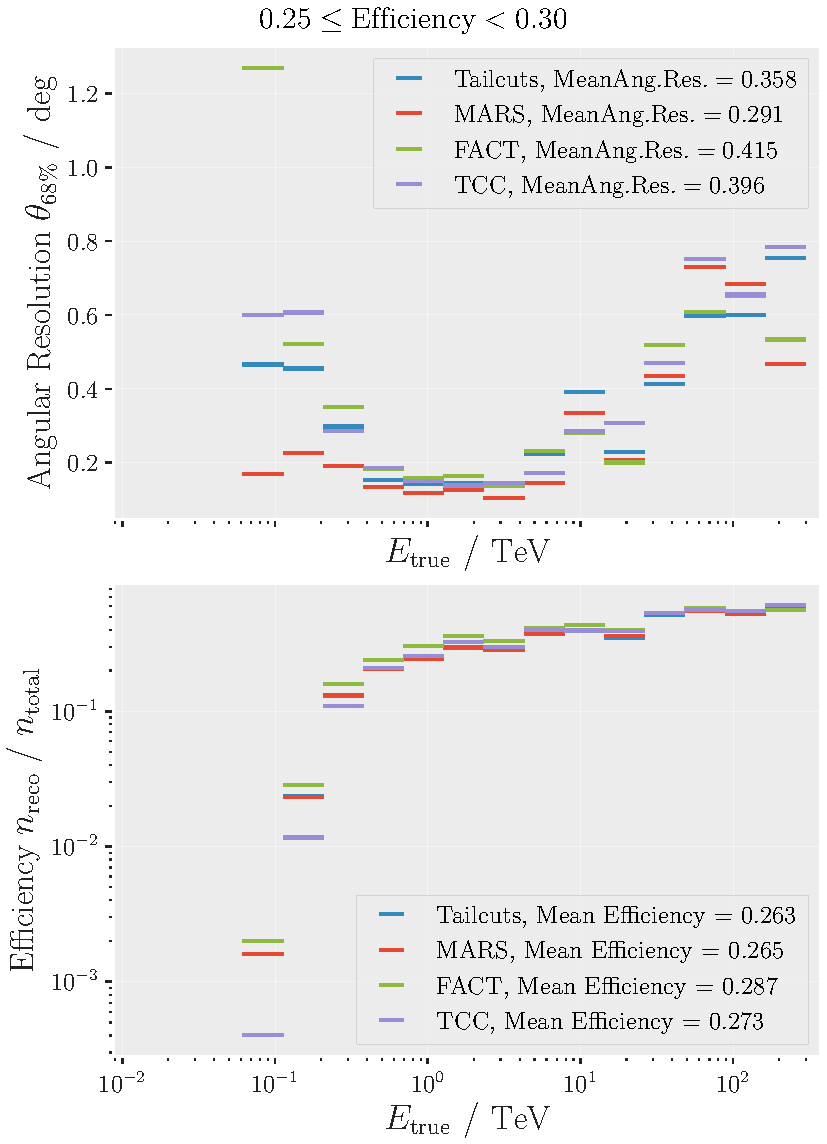
\includegraphics[width=\textwidth]{plots/ar_aeff/AR_Aeff_MST_0.25_0.30.pdf}
    \end{subfigure}
    \hfill
    \begin{subfigure}{0.48\textwidth}
        \centering
        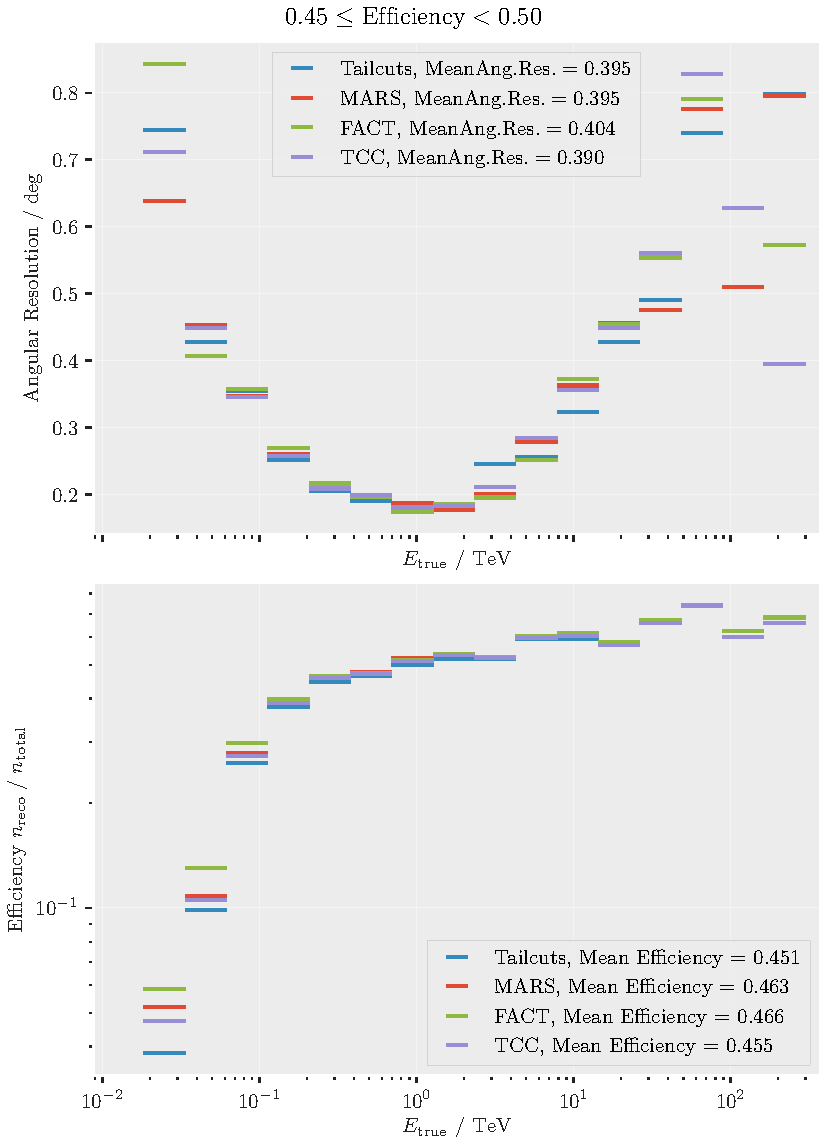
\includegraphics[width=\textwidth]{plots/ar_aeff/AR_Aeff_MST_0.45_0.50.pdf}
    \end{subfigure}
    \caption{Mean angular resolution and efficiency for the MST simulation binned per energy. Notice
    the decrease in the scattering of the mean angular resolution at medium to
    medium-high energies at higher efficiencies in the right plots.}
    \label{fig:efficiency_angres}
\end{figure}

Furthermore, the mean angular resolution is plotted against the efficiency in \autoref{fig:ar_vs_eff}.

\begin{figure}
    \centering
    \includegraphics[width=\textwidth]{build/ar_vs_eff.pdf}
    \caption{Angular resolution plotted against the efficiency.}
    \label{fig:ar_vs_eff}
\end{figure}


\section{Metrics of the cleaning algorithms}
\label{sec:metrics}
\glsreset{tp}\glsreset{fp}\glsreset{fn}\glsreset{tn}
Concerning the metrics, I first analyzed the parameter combinations of each cleaning algorithm. First,
the number of the \gls{tp}, \gls{fp}, \gls{fn} and \gls{tn} values is calculated per event. Then,
those values are summed up for each cleaning algorithm and the metrics are calculated as shown in
\autoref{tab:metrics}.

The metrics for each parameter combination are first compared for each cleaning algorithm respectively,
to determine the best setting within a set of parameter combinations. The results are then plotted in
\Autoref{fig:metrics_tail, fig:metrics_mars, fig:metrics_fact, fig:metrics_tcc}
and are shown with specific IDs they were given when the datasets were processed with \ctapipe.
This improves readability as opposed to writing out the full settings. The hyperparameters for the best performing
IDs of all algorithms are listed in \autoref{tab:best_parameters}.

While all settings perform well w.\,r.\,t., for example, the \gls{tnr}, one can see from the results, that for all cleaning
algorithms---except for \mars{}---, the best parameter combination is the one where the \gls{tpr}, the \gls{acc} and the \gls{ba}
are the highest. These settings are the ones that correspond to the highest efficiency. While this is true
for \tailcuts{}, \fact{} and \tcc{}, the metrics for \mars{} are an exception. The reason for that is, that when
looking at the corresponding mean angular resolution for the highest performing setting (ID~10), the value is
\(\SI{1.301}{\degree}\) (see \autoref{tab:angres}) and therefore an order of magnitude worse than the other algorithms. For better
comparison, I, therefore, choose the second highest performing setting (ID~15) with a mean angular
resolution of \(\SI{0.395}{\degree}\) to be the best candidate for further analysis.
The values for each respective metric and cleaning algorithm are listed in
\Autoref{tab:metrics_tail, tab:metrics_mars, tab:metrics_fact, tab:metrics_tcc} respectively, while
a comparison of the cleaners against each other is shown in \autoref{sec:comparison}.
\begin{table}
    \centering
    \caption{Results for the metrics of \tailcuts{}. One can see, that the best results are obtained
    for the settings with ID~47.}
    \label{tab:metrics_tail}
    \rowcolors{0}{white!92!black}{}
    \begin{tabular}{r S[table-format=1.4] S[table-format=1.4] S[table-format=1.4] S[table-format=1.4] S[table-format=1.4] S[table-format=1.4] S[table-format=1.4]}
        \hiderowcolors
        {ID} & \gls{tpr} & \gls{fpr} & \gls{tnr} & \gls{fnr} & \gls{ppv} & \gls{acc} & \gls{ba} \\
        \addlinespace[0.5em]
        \showrowcolors
        % \input{build/metrics_tail.txt} %% kinda broken atm
        118 & 0.0972 & 0.0000 & 1.0000 & 0.9028 & 1.0000 & 0.9256 & 0.5486 \\
        51 & 0.1231 & 0.0000 & 1.0000 & 0.8769 & 1.0000 & 0.9256 & 0.5615 \\
        140 & 0.1460 & 0.0000 & 1.0000 & 0.8540 & 1.0000 & 0.9256 & 0.5730 \\
        81 & 0.1854 & 0.0000 & 1.0000 & 0.8146 & 0.9997 & 0.9288 & 0.5927 \\
        47 & 0.2268 & 0.0000 & 1.0000 & 0.7732 & 0.9994 & 0.9332 & 0.6134 \\
    \end{tabular}
\end{table}

\begin{figure}
    \centering
    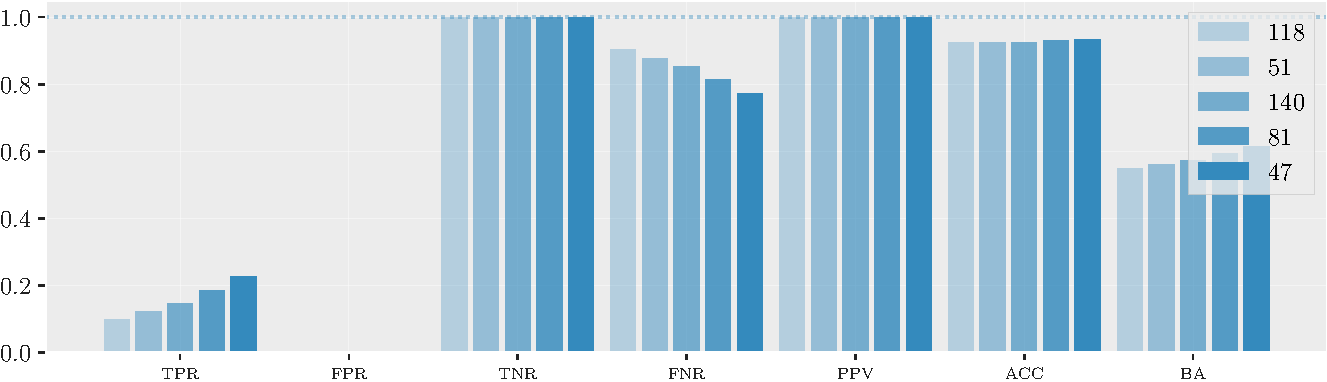
\includegraphics[width=\textwidth]{build/metrics_tailcuts.pdf}
    \caption{Metrics for \tailcuts{}. One can see that the cleaning setting with \wip{ID 47} performs
    best in terms of the true positive rate, accuracy and balanced accuracy, making it the best
    setting of the five parameter combinations.}
    \label{fig:metrics_tail}
\end{figure}

\begin{table}
    \centering
    \caption{Results for the metrics of \mars{}. The last row (ID~10) shows some increase in the \gls{fpr}
    and therefore some decrease in \gls{tnr} and a more significant decrease in the \gls{ppv} value. Since
    this specific parameter combination also corresponds to a mean angular resolution an order higher
    than the rest, I chose to select the second highest performing setting (ID~15) for further analysis
    instead.}
    \label{tab:metrics_mars}
    \rowcolors{0}{white!92!black}{}
    \begin{tabular}{r S[table-format=1.4] S[table-format=1.4] S[table-format=1.4] S[table-format=1.4] S[table-format=1.4] S[table-format=1.4] S[table-format=1.4]}
        \hiderowcolors
        ID & \gls{tpr} & \gls{fpr} & \gls{tnr} & \gls{fnr} & \gls{ppv} & \gls{acc} & \gls{ba} \\
        \addlinespace[0.5em]
        \showrowcolors
        \input{build/metrics_mars.txt}\\
    \end{tabular}
\end{table}

\begin{figure}
    \centering
    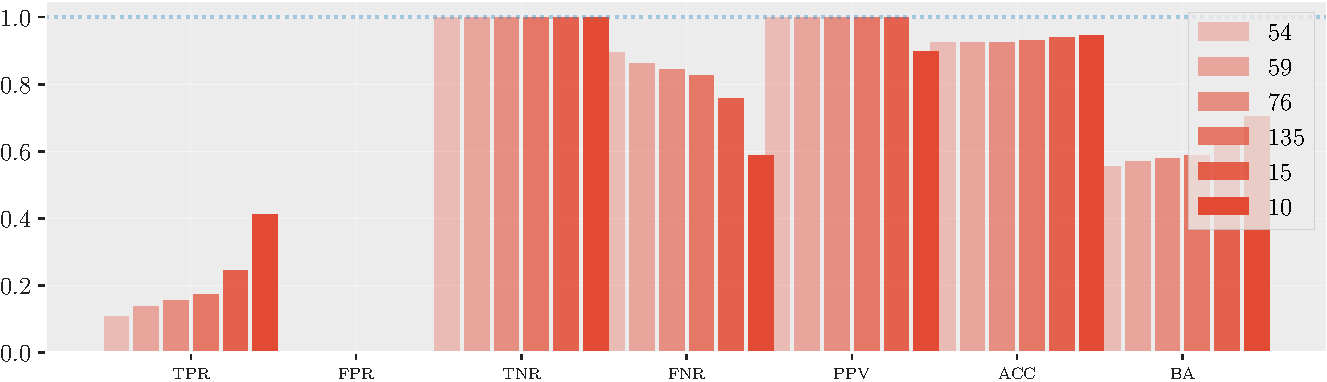
\includegraphics[width=\textwidth]{build/metrics_mars.pdf}
    \caption{Metrics for \mars{}. While ID~10 arguably performs best at first glance---albeit with a not
    insignificant decrease in the \gls{ppv} value---, I chose ID~15
    for further analysis, as its mean angular resolution is an order of magnitude better.}
    \label{fig:metrics_mars}
\end{figure}

\begin{table}
    \centering
    \caption{Results for the metrics of \fact{}. One can see, that the best results are obtained
    for the settings with ID~503.}
    \label{tab:metrics_fact}
    \rowcolors{0}{white!92!black}{}
    \begin{tabular}{r S[table-format=1.4] S[table-format=1.4] S[table-format=1.4] S[table-format=1.4] S[table-format=1.4] S[table-format=1.4] S[table-format=1.4]}
        \hiderowcolors
        ID & \gls{tpr} & \gls{fpr} & \gls{tnr} & \gls{fnr} & \gls{ppv} & \gls{acc} & \gls{ba} \\
        \addlinespace[0.5em]
        \showrowcolors
        \input{build/metrics_fact.txt}\\
    \end{tabular}
\end{table}

\begin{figure}
    \centering
    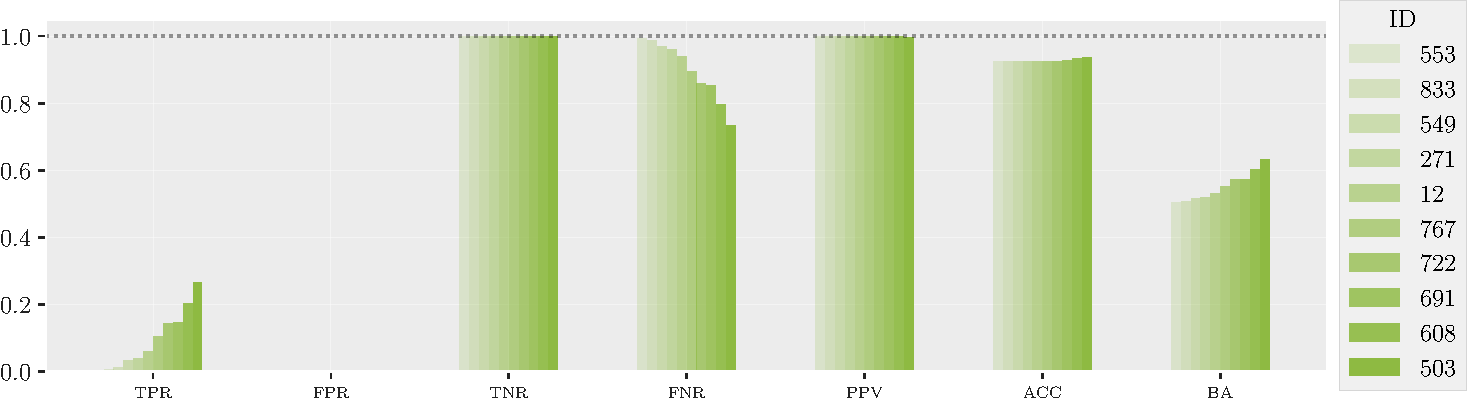
\includegraphics[width=\textwidth]{build/metrics_fact.pdf}
    \caption{Metrics for \fact{}. One can see that the cleaning setting with \wip{ID 503} performs
    best in terms of the number of true positives, accuracy and balanced accuracy, making it the best
    setting of the ten parameter combinations.}
    \label{fig:metrics_fact}
\end{figure}

\begin{table}
    \centering
    \caption{Results for the metrics of \tcc{}. One can see, that the best results are obtained
    for the settings with ID~807.}
    \label{tab:metrics_tcc}
    \rowcolors{0}{white!92!black}{}
    \begin{tabular}{r S[table-format=1.4] S[table-format=1.4] S[table-format=1.4] S[table-format=1.4] S[table-format=1.4] S[table-format=1.4] S[table-format=1.4] }
        \hiderowcolors
        ID & \gls{tpr} & \gls{fpr} & \gls{tnr} & \gls{fnr} & \gls{ppv} & \gls{acc} & \gls{ba} \\
        \addlinespace[0.5em]
        \showrowcolors
        \input{build/metrics_tcc.txt}\\
    \end{tabular}
\end{table}

\begin{figure}
    \centering
    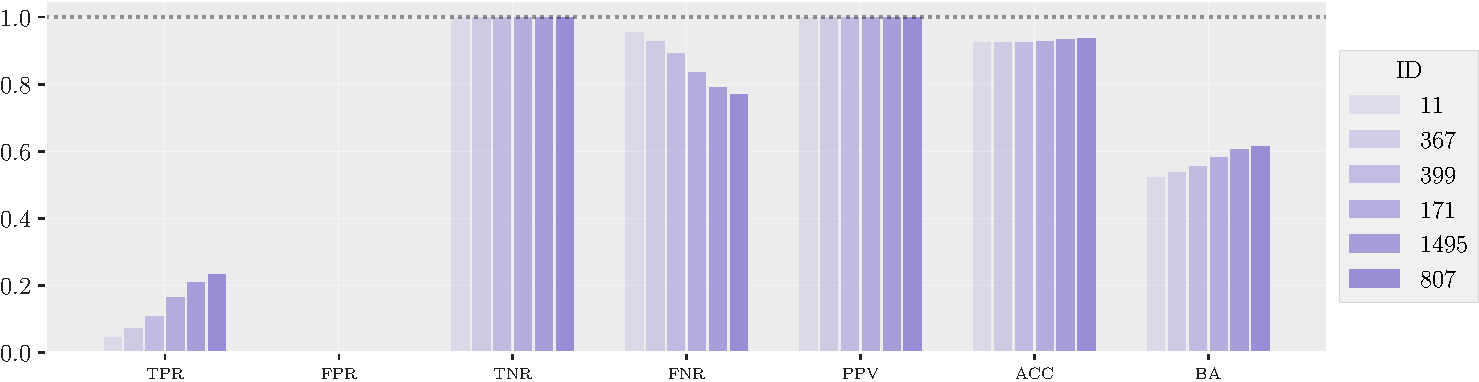
\includegraphics[width=\textwidth]{build/metrics_tcc.pdf}
    \caption{Metrics for the \tcc{}. One can see that the cleaning setting with \wip{ID 807} performs
    best in terms of the number of true positives, accuracy and balanced accuracy, making it the best
    setting of the six parameter combinations.}
    \label{fig:metrics_tcc}
\end{figure}

\begin{table}
    \centering
    \caption{Best performing IDs and the corresponding hyperparameters for each respective cleaner.
    Note, that, as discussed above, the best performing ID \wrt
    the metrics for \mars{} is, in fact, not the best, but the second best. This is because the mean angular resolution is
    an order of magnitude better for ID~15 than the one for ID~10. For better readability, the names
    of the algorithms are shortened. Listed are the core threshold \(Q_c\), the boundary threshold \(Q_b\),
    the minimum number of neighbors and where applicable the time limit \(t\) and core and boundary time limits
    \(t_c\) and \(t_b\).}
    \label{tab:best_parameters}
    \rowcolors{0}{white!92!black}{}
    \begin{tabular}{c S[table-format=2.0] S[table-format=1.3]
        S[table-format=1.3] S[table-format=1.0] S[table-format=2.1] S[table-format=2.1] S[table-format=2.1]}
        \hiderowcolors
        {Cleaning Algorithm} & {ID} & {\(Q_c \;/\; \si{\pe}\)} & {\(Q_b \;/\; \si{\pe}\)} & {Min. Neigh.} &
        {\(t \;/\; \si{\nano\second}\)} & {\(t_c \;/\; \si{\nano\second}\)} & {\(t_b \;/\; \si{\nano\second}\)} \\
        \addlinespace[0.5em]
        \showrowcolors
        Tailcuts &  47 & 6.200 & 4.650 & 2 &      &      &      \\
        MARS     &  15 & 6.700 & 4.467 & 1 &      &      &      \\
        FACT     & 503 & 6.700 & 3.350 & 1 & 12.0 &      &      \\
        TCC      & 807 & 6.700 & 4.467 & 1 &      & 15.0 & 12.0 \\
    \end{tabular}
\end{table}

\section{Performance compared to the default settings}
\label{sec:performance}

Now, with the best performing settings for each cleaner, it is resonable to compare
the performance to the default settings, that are implemented in the \ctapipe{} source code.

\section{Comparison of the cleaning algorithms}
\label{sec:comparison}

Because the cleaning algorithms in this work are the only ones that are implemented in the \ctapipe{}
source code as of writing this thesis, a comparison of the algorithms against each other seems to be
another feasible option. I once again decided to use the best-performing setting of each algorithm
and look at the metrics. The metrics of all four algorithms are shown in \autoref{fig:metrics_all}.
The corresponding values are listed in \autoref{tab:metrics_all}.

One can see, that \fact{} performs best in terms of \gls{tpr} and \gls{ba}, while \mars{} and
\tailcuts{} perform well on \gls{acc} and \gls{ppv} respectively. Overall, however, \fact{} seems
to be a good choice for cleaning since it performs reasonably well even on \gls{acc} and \gls{ppv}.


\begin{table}
    \centering
    \caption{Metrics for the best-performing settings of each cleaning algorithm. Out of these
    four algorithms, \fact{} performs best in terms of \gls{tpr} and \gls{ba}, while \mars{} and
    \tailcuts{} perform well on \gls{acc} and \gls{ppv} respectively. \fact{}, however, performs
    reasonably well in the scope of the resulting metrics of this work and is, therefore, a good
    overall choice for cleaning.}
    \label{tab:metrics_all}
    \rowcolors{0}{white!92!black}{}
    \begin{tabular}{c S[table-format=1.4] S[table-format=1.4] S[table-format=1.4]
        S[table-format=1.4] S[table-format=1.4] S[table-format=1.4] S[table-format=1.4]}
        \hiderowcolors
        {Cleaning Algorithm} & {\gls{tpr}} & {\gls{fpr}} & {\gls{tnr}} &
        {\gls{fnr}} & {\gls{ppv}} & {\gls{acc}} & {\gls{ba}} \\
        \addlinespace[0.5em]
        \showrowcolors
        Tailcuts & 0.2268 & 0.0000 & 1.0000 & 0.7732 & 0.9994 & 0.9332 & 0.6134 \\
        MARS     & 0.2433 & 0.0000 & 1.0000 & 0.7567 & 0.9985 & 0.9380 & 0.6216 \\
        FACT     & 0.2655 & 0.0000 & 1.0000 & 0.7345 & 0.9968 & 0.9369 & 0.6327 \\
        TCC      & 0.2314 & 0.0000 & 1.0000 & 0.7686 & 0.9989 & 0.9364 & 0.6157 \\
    \end{tabular}
\end{table}

\begin{figure}
    \centering
    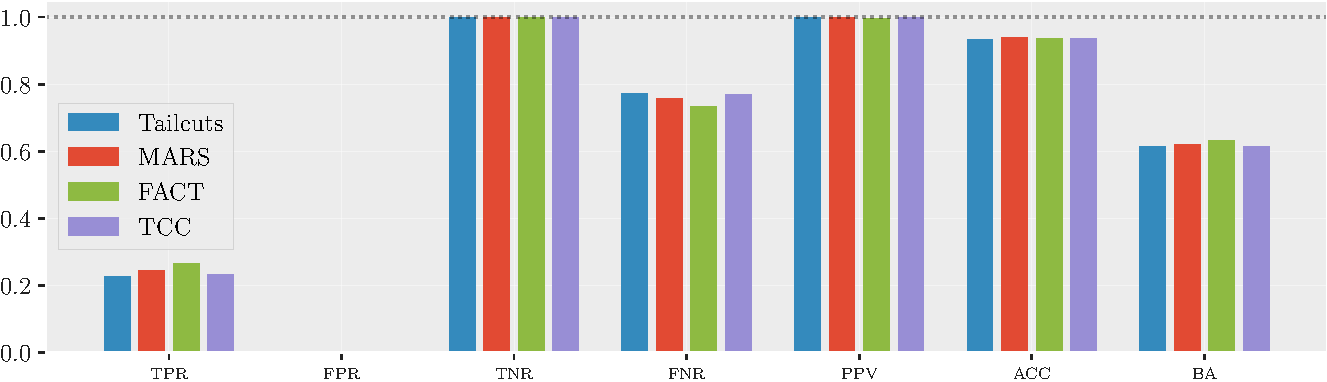
\includegraphics[width=\textwidth]{build/metrics_all.pdf}
    \caption{Bar plot visualizing the metrics for the best-performing settings of all four cleaning algorithms.}
    \label{fig:metrics_all}
\end{figure}